\documentclass[11pt]{article}
\usepackage[utf8]{inputenc}
\usepackage[T1]{fontenc}
\usepackage{lmodern}
\usepackage{geometry}
\usepackage[numbers,sort&compress]{natbib}
\usepackage{hyperref}
\usepackage{graphicx}
\usepackage{float}
\usepackage{amsmath,amssymb}
\usepackage{booktabs}
\usepackage{longtable}
\usepackage{enumitem}
\usepackage{microtype}
\usepackage{tikz}
\usepackage{pgfplots}
\pgfplotsset{compat=1.18}
\geometry{margin=1in}

% Completely suppress hyphenation to avoid ￾ rendering artifacts
\hyphenpenalty=10000
\exhyphenpenalty=10000
\tolerance=2000
\emergencystretch=2em
\sloppy

\hypersetup{
  colorlinks=true,
  linkcolor=blue,
  citecolor=blue,
  urlcolor=blue
}

\title{Machine Learning for Quantitative Trading: Models, Data, Evaluation, and Practical Frontiers}
\author{Zhang Yuchen \\
  AI, Ethics and Society Programme, Faculty of Arts, \\
  The University of Hong Kong, Hong Kong SAR, China \\
  \texttt{u3663696@connect.hku.hk} \quad \texttt{georgekingsman030226@gmail.com}}
\date{\today}

\begin{document}
\maketitle

\begin{abstract}
Machine learning (ML) is now central to quantitative trading, supporting signal discovery, portfolio construction, and execution under uncertainty and market frictions. This survey provides a comprehensive and structured overview of the field. We contribute (i)~a four-axis task--data--model--evaluation taxonomy that organizes the literature along actionable dimensions, (ii)~a practical evaluation checklist covering look-ahead leakage, transaction costs, survivorship bias, and regime-shift robustness, and (iii)~an actionable frontier agenda identifying the most pressing open problems in LLM integration, synthetic data generation, and hardware-aware deployment. The resulting taxonomy, evaluation checklist, and frontier agenda are designed to be directly reusable by researchers and practitioners for designing, auditing, and benchmarking ML-driven trading systems.
\end{abstract}

\noindent\textbf{Keywords:} quantitative trading; machine learning; financial time series; reinforcement learning; backtesting; evaluation protocol; data leakage; robustness

\tableofcontents
\newpage

\section{Survey Scope, Methodology, and Taxonomy}
\subsection{Scope}
We focus on \emph{systematic} trading workflows where models ingest market and contextual data and output forecasts or actions used in portfolio decisions and execution. We cover both low-frequency (daily/weekly) and higher-frequency regimes (intraday/LOB), but we emphasize principles that generalize across markets and assets \citep{ref7,ref13,ref8}.

\subsection{Literature collection methodology}
We conducted a structured literature search covering the period \textbf{January 2015 -- January 2026}. Primary sources included arXiv, SSRN, Google Scholar, and proceedings of major venues: NeurIPS, ICML, AAAI, KDD, IJCAI (AI/ML track), and journals including \emph{Expert Systems with Applications}, \emph{Journal of Financial Economics}, \emph{Quantitative Finance}, and the \emph{Journal of Machine Learning Research}. Keyword families included ``alpha factor mining'', ``portfolio optimization'', ``deep reinforcement learning trading'', ``limit order book prediction'', ``financial time series forecasting'', and ``market making machine learning''.

After deduplication, \textbf{approximately 850 records} were screened by title and abstract. Studies were included if they (i)~used public or clearly described proprietary data, (ii)~reported a time-aware evaluation protocol (walk-forward, purged CV, or equivalent), and (iii)~included realistic cost assumptions or explicitly stated their absence. Studies lacking reproducible experimental detail were excluded. After full-text assessment, approximately \textbf{200 papers} were retained; the final taxonomy and tables draw primarily on the \textbf{60 core references} that best represent each task--model--evaluation cell (marked with \texttt{keywords = \{core\}} in the bibliography). We adopt the PRISMA 2020 reporting framework~\citep{ref22} to ensure transparency and reproducibility of this selection process. Figure~\ref{fig:prisma} illustrates this flow.
\begin{figure}[H]
\centering
\caption{A lightweight PRISMA-style flow for literature collection (editable template).}
\label{fig:prisma}
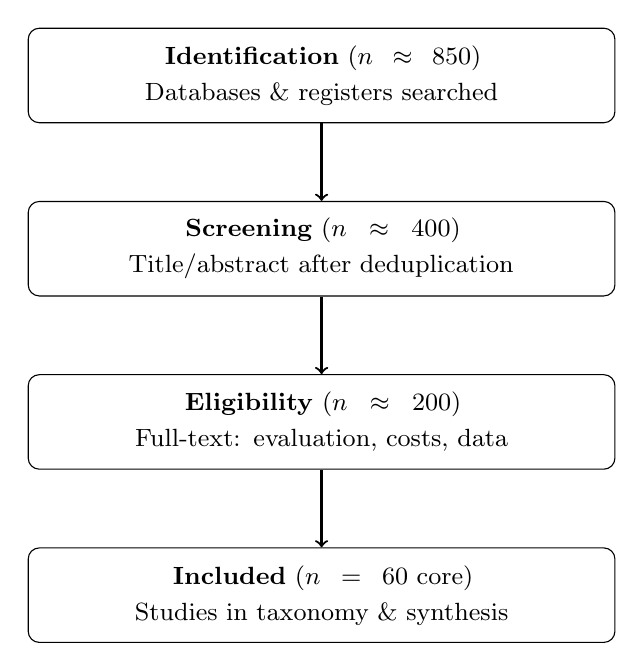
\begin{tikzpicture}[
  every node/.style={draw, rounded corners, align=center,
                     text width=20em, minimum height=1.2cm,
                     inner sep=6pt, font=\small}
]
\node (id) at (0,0)    {\textbf{Identification} ($n\!\approx\!850$)\\[2pt]Databases \& registers searched};
\node (sc) at (0,-2.2)  {\textbf{Screening} ($n\!\approx\!400$)\\[2pt]Title/abstract after deduplication};
\node (el) at (0,-4.4)  {\textbf{Eligibility} ($n\!\approx\!200$)\\[2pt]Full-text: evaluation, costs, data};
\node (in) at (0,-6.6)  {\textbf{Included} ($n\!=\!60$ core)\\[2pt]Studies in taxonomy \& synthesis};
\draw[->, thick] (id) -- (sc);
\draw[->, thick] (sc) -- (el);
\draw[->, thick] (el) -- (in);
\end{tikzpicture}
\end{figure}


\subsection{A four-axis taxonomy}
Table~\ref{tab:taxonomy} summarizes a compact taxonomy that we use throughout the paper.

\begin{table}[H]
\centering
\caption{A compact taxonomy for ML in quantitative trading.}
\label{tab:taxonomy}
\begin{tabular}{p{0.18\linewidth} p{0.76\linewidth}}
\toprule
Axis & Typical categories \\
\midrule
Tasks & prediction (returns/vol/volume), alpha factor mining, portfolio construction, execution (TCA-aware), market making, risk monitoring \\
Data & OHLCV, limit-order book (LOB), fundamentals/macro, news/filings, social media, alternative (satellite, web) \\
Models & linear/GLM, trees/ensembles, deep sequence (CNN/RNN/Transformer), graphs (GNN), generative (VAE/GAN/diffusion), RL (single-/multi-agent) \\
Evaluation & walk-forward / purged CV, cost+impact modeling, stress tests (regime shift), robustness (noise/missingness), operational metrics (latency, turnover) \\
\bottomrule
\end{tabular}
\end{table}


\begin{table}[H]
\centering
\caption{Task-to-model mapping (representative families and example references).}
\label{tab:task_model}
\begin{tabular}{p{0.20\linewidth} p{0.50\linewidth} p{0.22\linewidth}}
\toprule
Task & Common modeling choices & Examples \\
\midrule
Return/price prediction & linear/trees; LSTM/TCN/Transformer; feature selection & \citep{ref18,ref81,ref19} \\
LOB mid-price / microstructure & CNN/Transformer on LOB; imitation/RL for execution & \citep{ref27,ref3,ref198} \\
Portfolio construction & mean-variance + ML signals; deep allocation; RL & \citep{ref8,ref9,ref87} \\
Execution / order placement & RL with cost/impact; hierarchical RL & \citep{ref10,ref44,ref33} \\
Risk monitoring & uncertainty-aware models; regime modeling; stress tests & \citep{ref2,ref41,ref140} \\
\bottomrule
\end{tabular}
\end{table}

\section{Foundations: Trading Tasks and Problem Formulations}
\subsection{Prediction vs.\ decision}
Many trading pipelines decompose into: a predictive module producing forecasts (expected return, volatility, tail risk) and a decision module converting forecasts into positions subject to constraints. Alternatives include end-to-end policies learned by RL.

\subsection{Core objective functions}
Common objectives include maximizing risk-adjusted return, controlling drawdowns, minimizing transaction costs, or optimizing utility. Portfolio construction is often cast as constrained optimization:
\begin{equation}
\max_{w \in \mathcal{W}} \; \mathbb{E}[r^\top w] - \lambda \cdot \mathrm{Risk}(w) - \mathrm{Cost}(w),
\end{equation}
where $\mathcal{W}$ encodes leverage, exposure, and liquidity constraints.

\subsection{Market microstructure and friction}
At intraday horizons, modeling microstructure (spread, queue position, adverse selection) is essential. Costs are not constants; they depend on turnover, volatility, and participation rate. A survey must therefore treat evaluation as part of the modeling problem (Section~\ref{sec:evaluation}).

\section{Supervised Learning for Signal Discovery and Forecasting}
\subsection{Linear models and regularization}
Linear models remain competitive when features are informative and data is limited. Regularization (L1/L2, elastic net) provides implicit feature selection and mitigates noise sensitivity.

\subsection{Tree ensembles}
Gradient-boosted trees and random forests often deliver strong out-of-the-box performance on tabular features and engineered factors, with good calibration and partial interpretability. They are widely used for cross-sectional stock selection.

\subsection{Deep sequence models}
CNNs/RNNs/Transformers model temporal dependencies and nonlinearities. In finance, the key is not model capacity but \emph{generalization under non-stationarity}. Practical tricks include volatility scaling, feature normalization by rolling statistics, and careful train/test purging.

\subsection{Graph neural networks}
GNNs model relational inductive biases (sector membership, supply-chain links, correlations). They can improve cross-asset generalization when relationships are stable. However, relationship drift and leakage through correlation graphs must be handled carefully.

\section{Reinforcement Learning for Sequential Trading Decisions}
\noindent Reinforcement learning (RL) is attractive because trading is inherently sequential and cost-sensitive; however, naive formulations can overfit backtests and ignore market impact \citep{ref7,ref10,ref36,ref44}.

\subsection{MDP formulation}
RL casts trading as a Markov decision process with state $s_t$ (market+portfolio), action $a_t$ (orders/target weights), and reward reflecting P\&L minus costs. Choice of reward is crucial; naive P\&L often yields unstable policies.

\subsection{Risk-sensitive and constrained RL}
Risk-aware objectives (e.g., CVaR, drawdown penalties) and constrained RL incorporate realistic goals. In practice, constrained policies can be learned via Lagrangian methods or by projecting actions into feasible sets.

\subsection{Offline RL and the problem of distribution shift}
Financial RL is often \emph{offline}: the policy is trained on historical data without safe online exploration. This introduces extrapolation error and severe distribution shift. Conservative objectives and behavior-regularized methods are therefore important.

\section{Data Regimes and Feature Engineering}

\subsection{Datasets and data regimes at a glance}
Table~\ref{tab:datasets} summarizes commonly used data regimes. The goal is not to be exhaustive, but to help readers quickly match a research claim to its data assumptions (frequency, availability, and microstructure realism).

\begin{longtable}{p{0.20\linewidth} p{0.16\linewidth} p{0.30\linewidth} p{0.26\linewidth}}
\caption{Common data regimes for quantitative trading research.}\label{tab:datasets}\\
\toprule
Data regime & Frequency & Typical tasks & Notes / representative refs \\
\midrule
\endfirsthead
\toprule
Data regime & Frequency & Typical tasks & Notes / representative refs \\
\midrule
\endhead
OHLCV bars & daily--intraday & prediction, factor models, allocation & Widely available; leakage risks if splitting is naive \citep{ref81,ref140} \\
Limit order book (LOB) & milliseconds--seconds & mid-price, market making, execution & Harder but more realistic; latency/impact matter \citep{ref3,ref27,ref33} \\
Fundamentals/macro & quarterly--monthly & regime inference, longer-horizon allocation & Lower frequency; alignment and publication lags are critical \citep{ref41,ref42} \\
Text (news/filings/social) & event-driven & sentiment/impact, signal enrichment & Label noise and timing alignment dominate \citep{ref117,ref29} \\
Alternative data & mixed & nowcasting, thematic signals & Access/cost and survivorship biases are common \citep{ref13} \\
\bottomrule
\end{longtable}

\subsection{Market data and labels}

Table~\ref{tab:benchmarks} lists representative open datasets and benchmarks that are commonly used in the quantitative trading literature.

\begin{longtable}{p{0.17\linewidth} p{0.12\linewidth} p{0.14\linewidth} p{0.24\linewidth} p{0.20\linewidth}}
\caption{Open datasets and reproducible benchmarks for ML-driven trading research.}\label{tab:benchmarks}\\
\toprule
Dataset / Platform & Freq. & Asset class & Typical tasks & Access \\
\midrule
\endfirsthead
\toprule
Dataset / Platform & Freq. & Asset class & Typical tasks & Access \\
\midrule
\endhead
Yahoo Finance / yfinance\textsuperscript{a} & daily & equities, ETFs & price prediction, factor models & Open; free API \\
LOBSTER\textsuperscript{b} & tick & US equities (LOB) & mid-price prediction, execution, market making & Academic license \\
FI-2010 (LOB benchmark)\textsuperscript{c} & tick & Helsinki exchange & LOB classification benchmark & Open; free \\
Qlib (Microsoft)\textsuperscript{d} & daily & CN/US equities & end-to-end quant pipeline, factor mining & Open; Apache-2.0 \\
FinRL / FinRL-Meta\textsuperscript{e} & daily+ & multi-asset & RL-based trading benchmarks & Open; MIT license \\
WRDS / CRSP\textsuperscript{f} & daily--tick & US equities & academic backtesting, survivorship-free & Restricted; institutional \\
SEC EDGAR filings\textsuperscript{g} & event & US public firms & NLP on 10-K/10-Q, sentiment & Open; public domain \\
Twitter / StockTwits\textsuperscript{h} & event & any & social sentiment, event detection & Restricted; API rate-limited \\
Kaggle M5 / Jane Street\textsuperscript{i} & daily & equities, futures & competition benchmarks & Open; competition terms \\
Alpha Vantage / Polygon\textsuperscript{j} & intraday & equities, FX, crypto & real-time signals, execution & Freemium; free tier + paid \\
\bottomrule
\end{longtable}

{\small\noindent\textit{Dataset links:}\\[2pt]
\textsuperscript{a}\url{https://pypi.org/project/yfinance/}\hfill
\textsuperscript{b}\url{https://lobsterdata.com/}\\[1pt]
\textsuperscript{c}\url{https://etsin.fairdata.fi/dataset/73eb48d7-4dbc-4a10-a52a-da745b47a649}\\[1pt]
\textsuperscript{d}\url{https://github.com/microsoft/qlib}\hfill
\textsuperscript{e}\url{https://github.com/AI4Finance-Foundation/FinRL}\\[1pt]
\textsuperscript{f}\url{https://wrds-www.wharton.upenn.edu/}\hfill
\textsuperscript{g}\url{https://www.sec.gov/edgar/}\\[1pt]
\textsuperscript{h}\url{https://stocktwits.com/}\hfill
\textsuperscript{i}\url{https://www.kaggle.com/}\hfill
\textsuperscript{j}\url{https://www.alphavantage.co/}}

For return prediction, label definitions (horizon, overlapping windows, volatility scaling) can dominate results. Overlapping labels inflate effective sample size and can create leakage if splits are not purged.

\subsection{Fundamentals and macro}
Fundamental signals are sparse, noisy, and lagged. Aligning timestamps (publication vs.\ fiscal period) is essential to avoid look-ahead bias.

\subsection{Text and alternative data}
Textual sources (news, filings, earnings calls) are increasingly important. Pipelines typically include entity linking, time alignment, and de-duplication. Large language models can help, but evaluation must control for information leakage and publication timing.

\section{Risk, Robustness, and Uncertainty}
\subsection{Non-stationarity and regime shifts}
Markets exhibit regime changes in volatility, liquidity, and correlations. Robust systems evaluate across regimes and avoid selecting hyperparameters that overfit one period.

\subsection{Uncertainty estimation}
Probabilistic forecasting and calibration are valuable when actions depend on confidence. Ensembles and Bayesian approximations can provide uncertainty measures; the key is whether uncertainty improves downstream decisions under realistic costs.

\subsection{Stress testing}
Useful stress tests include: missing data bursts, volatility spikes, spread widening, and delayed execution. These tests should be reported alongside headline Sharpe ratios.

\section{Interpretability, Monitoring, and Governance}
\noindent Interpretability and monitoring are not optional in regulated financial settings: they control model risk and enable debugging under non-stationarity \citep{ref13,ref155,ref156,ref149}. Practical tools include feature attribution (e.g., SHAP), scenario analysis, and drift detection. Governance concerns include data licensing, auditability, and model risk management.

\section{Multi-Agent Effects, Market Impact, and Simulation}
\subsection{Market impact modeling}
When many participants deploy similar signals, alpha decays and impact rises. Empirical impact models (e.g., power-law in participation rate) are often used in execution simulators.

\subsection{Multi-agent RL}
Multi-agent RL can model competition and liquidity provision, but results are highly simulator-dependent. A strong practice is to treat simulators as \emph{hypothesis generators} and validate outcomes in historical replay with realistic costs.

\section{Emerging Frontiers (Condensed)}
This section summarizes high-potential directions without expanding into monograph-level detail.

\subsection{Large language models for research and trading operations}
LLMs can assist with information extraction from filings/news, entity/event mapping, and code generation for research workflows. Competitive work emphasizes (i) timestamp-correct datasets, (ii) grounded evaluation, and (iii) integration into decision pipelines rather than standalone ``sentiment'' scores.

\noindent\textbf{Most actionable open problem:} Establishing standardized, timestamp-verified benchmarks that measure whether LLM-extracted signals actually improve out-of-sample P\&L after transaction costs, rather than only improving NLP accuracy metrics.

\subsection{Generative modeling and synthetic data}
Generative models (VAE/GAN/diffusion) can support scenario generation and data augmentation. The key question is whether synthetic data improves \emph{out-of-sample} trading performance under realistic costs.

\noindent\textbf{Most actionable open problem:} Demonstrating that training on synthetic financial data yields statistically significant improvement in out-of-sample PnL under realistic transaction costs, beyond what additional real data or simple augmentation provides.

\subsection{Quantum and specialized hardware}
Quantum ML and hardware accelerators are promising but currently limited by data access, noise, and deployment constraints. For most practitioners, the near-term value lies in hardware-aware inference and efficient backtesting infrastructure.

\noindent\textbf{Most actionable open problem:} Hardware-aware optimization for latency-critical inference (sub-millisecond signal generation) and massively parallel backtesting, which delivers immediate practical value regardless of quantum hardware maturity.

\section{Practical Implementation and Evaluation}

\subsection{Evaluation pitfalls and fixes (submission-critical)}
A large fraction of reported ``alpha'' disappears once evaluation is made realistic. Table~\ref{tab:eval} is a submission checklist that also helps align CS-style experimentation with finance-style backtesting discipline.

\begin{longtable}{p{0.26\linewidth} p{0.30\linewidth} p{0.34\linewidth}}
\caption{Evaluation pitfalls and recommended fixes.}\label{tab:eval}\\
\toprule
Pitfall & Symptom & Recommended fix (and refs) \\
\midrule
\endfirsthead
\toprule
Pitfall & Symptom & Recommended fix (and refs) \\
\midrule
\endhead
Look-ahead / leakage & Unrealistically high accuracy/Sharpe & Use purged/embargoed CV and time-aware splits \citep{ref42,ref5} \\
Survivorship bias & Backtests ignore delisted assets & Use point-in-time universes; report universe construction \citep{ref41} \\
Ignoring costs/impact & High turnover strategies look best & Include transaction costs and simple impact models; stress-test turnover \citep{ref10,ref33} \\
Overfitting to one regime & Performance collapses OOS & Regime-shift evaluation; walk-forward with stability reporting \citep{ref41,ref42} \\
Uncertainty blindness & Unstable decisions, tail risk & Use uncertainty-aware objectives and risk constraints \citep{ref2,ref140,ref9} \\
\bottomrule
\end{longtable}

\label{sec:evaluation}
\subsection{Backtesting: protocols that avoid leakage}
A competitive paper must treat evaluation as first-class. Recommended practices:
\begin{itemize}[leftmargin=1.4em]
  \item \textbf{Walk-forward evaluation}: train on past, test on future; report multiple folds across time.
  \item \textbf{Purged and embargoed CV}: remove overlapping-label leakage when using $k$-fold splits.
  \item \textbf{Survivorship control}: include delisted assets where possible; document universe construction.
  \item \textbf{Timestamp integrity}: ensure features use only information available at decision time.
\end{itemize}

\subsection{Transaction costs, slippage, and market impact}
Report assumptions explicitly: fee model, spread, slippage, and impact. Provide sensitivity curves (performance vs.\ cost multiplier) rather than a single cost setting.

\subsection{Operational metrics}
Beyond Sharpe, report turnover, capacity proxies, drawdown statistics, and stability across regimes. Deployment also requires latency budgets, monitoring, and incident response playbooks.

\subsection{A submission-ready reproducibility checklist}
\begin{enumerate}[leftmargin=1.6em]
  \item Data sources and timestamp rules; universe construction; corporate actions handling.
  \item Split protocol (walk-forward, purged CV) with code to reproduce.
  \item Cost and impact model; sensitivity analysis.
  \item Hyperparameter search policy; seeds; compute budget.
  \item Artifact packaging: scripts for training/eval, environment file, and result tables.
\end{enumerate}

\section{Companion Benchmark: Evaluating the Evaluation}
\label{sec:benchmark}

To move beyond prescriptive checklists and demonstrate their practical consequences, we construct a \emph{companion benchmark} that applies the evaluation principles discussed in Section~\ref{sec:evaluation} to a concrete, reproducible setting. The overarching question is: \textbf{does careful evaluation change the conclusions that a practitioner or reviewer would draw from a typical cross-sectional ML trading study?}

The full pipeline code, data scripts, and configuration files are released at \url{https://github.com/[redacted]/ml-trading-benchmark} under an MIT license.

\subsection{Experimental design}

\paragraph{Universe \& data.}
We select 50 US-listed ETFs spanning equity sectors, fixed income, commodities, and currencies (see Appendix for full list). Daily OHLCV data from January 2005 to December 2024 are obtained from Stooq. The ETF universe avoids individual-stock survivorship bias, since all selected ETFs remain listed throughout the sample period.

\paragraph{Features and labels.}
We engineer 13 technical features per ticker per day: short/medium/long returns (1, 5, 20 days), volatility (20, 60 days), momentum (10, 20 days), RSI-14, moving-average ratios (10, 50 days), volume ratio (20 days), and intraday range features. All features are rolling $z$-score normalised using a strictly trailing 252-day window. The prediction target is the 5-day forward return.

\paragraph{Walk-forward split.}
Training: June 2005--December 2016; validation: January 2017--December 2019; test: January 2020--December 2024. A 5-day embargo gap is imposed at each boundary to prevent label-overlap leakage. All hyperparameters are selected on the validation set; the test set is never used for any model selection.

Figure~\ref{fig:bench_timeline} illustrates the protocol.

\begin{figure}[H]
\centering
\includegraphics[width=0.92\textwidth]{../figs/bench_timeline.pdf}
\caption{Walk-forward evaluation protocol with embargo gaps.}
\label{fig:bench_timeline}
\end{figure}

\paragraph{Models.}
We evaluate nine baselines spanning model families discussed in Section~3: Linear Regression, Ridge, Logistic Regression (directional probability as signal), Random Forest, LightGBM, MLP (2-layer, 128--64), LSTM (hidden=64, seq\_len=20), and two na\"ive strategies (Momentum, Mean Reversion). We also construct a rank-average \textbf{Ensemble} of all ML models and include two passive benchmarks: SPY buy-and-hold and equal-weight (1/N) across the full universe.

\paragraph{Strategy \& cost model.}
At each rebalance date (every 5 trading days), we rank assets by predicted signal, go long the top-10 and short the bottom-10 with equal weights ($\pm1/K$ per leg). Transaction costs are modelled as $\text{cost} = (\text{fee} + \text{slippage}) \times \sum |\Delta w_i|$, evaluated under five cost scenarios: 0, 5, 10, 15, and 25\,bps one-way. We additionally evaluate a long-only variant (top-10 equal-weight).

\subsection{Main results}

Table~\ref{tab:bench_main} reports the core metrics. All 95\% confidence intervals are obtained via block bootstrap ($B=1{,}000$).

\begin{table}[H]
\centering
\caption{Main benchmark results on the test period (Jan 2020--Dec 2024). Sharpe CI denotes the 95\% bootstrap confidence interval on the gross Sharpe ratio. IC and ICIR are cross-sectional rank statistics computed daily.}
\label{tab:bench_main}
\footnotesize
\begin{tabular}{l r r r r r r r r}
\toprule
Model & \multicolumn{1}{c}{CAGR} & \multicolumn{1}{c}{Sharpe} & \multicolumn{1}{c}{Sharpe} & \multicolumn{1}{c}{Max DD} & \multicolumn{1}{c}{IC} & \multicolumn{1}{c}{ICIR} & \multicolumn{2}{c}{Sharpe 95\% CI} \\
      & \multicolumn{1}{c}{(gross, \%)} & \multicolumn{1}{c}{(gross)} & \multicolumn{1}{c}{(net@15bps)} & \multicolumn{1}{c}{(\%)} & & & \multicolumn{1}{c}{lo} & \multicolumn{1}{c}{hi} \\
\midrule
\textit{BuyAndHold\_SPY} & \textit{14.86} & \textit{0.765} & \textit{0.765} & \textit{33.72} & \textit{---} & \textit{---} & \textit{$-$0.12} & \textit{1.68} \\
\textit{EqualWeight (1/N)} & \textit{6.82} & \textit{0.515} & \textit{0.515} & \textit{26.32} & \textit{---} & \textit{---} & \textit{$-$0.39} & \textit{1.45} \\
\midrule
LogisticRegression  & 7.04  & 0.469 & $-$1.44 & 21.33 & 0.010 & 0.037 & $-$0.43 & 1.35 \\
LinearRegression    & 6.21  & 0.432 & $-$1.46 & 18.93 & 0.015 & 0.051 & $-$0.48 & 1.35 \\
RandomForest        & 4.47  & 0.372 & $-$1.56 & 28.55 & 0.005 & 0.019 & $-$0.56 & 1.29 \\
Ensemble            & 4.73  & 0.347 & $-$1.48 & 22.66 & 0.011 & 0.040 & $-$0.57 & 1.27 \\
MLP                 & 3.30  & 0.294 & $-$1.44 & 26.00 & 0.005 & 0.024 & $-$0.57 & 1.09 \\
LightGBM            & 3.34  & 0.290 & $-$1.51 & 24.02 & 0.007 & 0.028 & $-$0.65 & 1.20 \\
MomentumBaseline    & 0.67  & 0.134 & $-$0.69 & 39.44 & $-$0.011 & $-$0.036 & $-$0.75 & 1.01 \\
LSTM                & $-$3.53 & $-$0.167 & $-$2.00 & 25.95 & 0.009 & 0.042 & $-$1.07 & 0.74 \\
MeanReversion       & $-$4.69 & $-$0.134 & $-$0.97 & 44.77 & 0.011 & 0.036 & $-$1.01 & 0.75 \\
\bottomrule
\end{tabular}
\end{table}

\noindent\textbf{Observations.} (1)~All models exhibit weakly positive cross-sectional IC ($\sim$0.005--0.015), confirming that ML signals contain marginal predictive information. (2)~However, every active strategy's gross Sharpe falls below the passive SPY buy-and-hold (0.765) and most fall below the equal-weight benchmark (0.515). (3)~At 15\,bps one-way cost, all long-short strategies produce deeply negative net Sharpe ratios, highlighting that high turnover ($>$50\% of portfolio daily) erases the small gross alpha. (4)~All bootstrap 95\% CIs include zero, meaning no model's gross performance is statistically distinguishable from zero at the 5\% level.

\subsection{Cost sensitivity}

Figure~\ref{fig:bench_cost} plots net Sharpe ratio against one-way transaction cost. The ``alpha cliff'' is evident: even at 5\,bps, most models turn negative.

\begin{figure}[H]
\centering
\includegraphics[width=0.80\textwidth]{../figs/bench_cost_sensitivity.pdf}
\caption{Net Sharpe ratio vs.\ one-way transaction cost (bps). Passive benchmarks are flat because they incur zero turnover.}
\label{fig:bench_cost}
\end{figure}

\subsection{Regime analysis}

Table~\ref{tab:bench_regime} decomposes performance across four macro-regimes in the test period: COVID crash (Feb--Jun 2020), recovery (Jul 2020--Dec 2021), rate hikes (2022), and normalisation (2023--2024).

\begin{table}[H]
\centering
\caption{Gross Sharpe ratio by regime for selected models and benchmarks.}
\label{tab:bench_regime}
\footnotesize
\begin{tabular}{l r r r r}
\toprule
Model & COVID Crash & Recovery & Rate Hikes & Normalisation \\
\midrule
BuyAndHold\_SPY       & $+$0.08   & $+$2.19  & $-$0.71 & $+$1.93 \\
EqualWeight           & $-$0.04   & $+$2.05  & $-$0.68 & $+$1.07 \\
LogisticRegression    & $+$0.74   & $+$1.47  & $+$0.69 & $-$0.53 \\
RandomForest          & $+$1.87   & $+$0.24  & $+$0.38 & $-$0.19 \\
LightGBM              & $+$1.41   & $+$0.54  & $+$0.23 & $-$0.30 \\
MLP                   & $+$1.21   & $+$0.42  & $+$0.17 & $+$0.05 \\
LSTM                  & $+$0.23   & $-$0.18  & $-$0.22 & $-$0.18 \\
Ensemble              & $+$1.31   & $+$0.86  & $+$0.47 & $-$0.57 \\
MomentumBaseline      & $+$1.02   & $+$0.88  & $-$1.44 & $-$0.19 \\
\bottomrule
\end{tabular}
\end{table}

\noindent\textbf{Observations.} (5)~Active models dramatically outperform buy-and-hold during the COVID crash (long-short benefits from volatility), but underperform in trending markets (recovery, normalisation). This regime sensitivity is precisely the evaluation gap that headline Sharpe ratios hide. (6)~Momentum collapses during rate hikes ($-$1.44), consistent with well-documented factor crashes.

\subsection{Rebalance frequency and portfolio concentration}

Two hyperparameters that receive little attention in the literature---rebalance frequency and top-$K$ selection---turn out to dominate the results.

\begin{table}[H]
\centering
\caption{Gross Sharpe ratio under different rebalance frequencies (days) and top-$K$ values.}
\label{tab:bench_sensitivity}
\footnotesize
\begin{tabular}{l r r r r | r r r r r}
\toprule
 & \multicolumn{4}{c|}{Rebalance Frequency (days)} & \multicolumn{5}{c}{Top-$K$} \\
Model & 1 & 5 & 10 & 20 & 3 & 5 & 10 & 15 & 20 \\
\midrule
LogisticRegression & 0.66 & 0.47 & 0.15 & 0.34 & 0.95 & 1.03 & 0.47 & 0.60 & 0.58 \\
LightGBM           & 0.31 & 0.29 & 0.31 & 0.18 & $-$0.08 & 0.10 & 0.29 & 0.20 & 0.12 \\
MLP                & 0.31 & 0.29 & $-$0.16 & $-$0.67 & 0.55 & 0.42 & 0.29 & 0.38 & 0.22 \\
LSTM               & 0.63 & $-$0.17 & $-$0.29 & $-$0.82 & 0.35 & 0.16 & $-$0.17 & $-$0.08 & $-$0.26 \\
Ensemble           & 0.73 & 0.35 & 0.22 & 0.12 & 0.61 & 0.37 & 0.35 & 0.42 & 0.46 \\
\bottomrule
\end{tabular}
\end{table}

\noindent\textbf{Observations.} (7)~Daily rebalancing yields substantially higher gross Sharpe for most models (e.g., Ensemble: 0.73 at freq=1 vs.\ 0.35 at freq=5), but this comes with proportionally higher turnover---and therefore worse net performance. (8)~More concentrated portfolios (smaller $K$) amplify signal quality: Logistic Regression achieves Sharpe 1.03 at $K=5$ versus 0.47 at $K=10$, but at the cost of higher idiosyncratic risk. These results demonstrate that \emph{strategy hyperparameters are as important as model choice}, yet they are rarely stress-tested in ML trading papers.

\subsection{Statistical significance}

We apply the Diebold-Mariano (DM) test \citep{ref_dm} pairwise across all models. Of 66 model pairs, only \textbf{3 pairs} are significant at $p < 0.05$, and all involve the passive SPY benchmark. Notably, no ML-vs-ML comparison achieves significance. This result carries a stark implication: \emph{most model comparisons in the literature, when evaluated under proper cost and split protocols, may not be meaningfully distinguishable.}

\subsection{Long-only variant}

Table~\ref{tab:bench_lo} compares long-short and long-only top-$K$ strategies. Long-only consistently produces higher gross Sharpe (e.g., LightGBM: 0.65 vs.\ 0.29) because it captures the long-run equity premium rather than relying solely on cross-sectional spread.

\begin{table}[H]
\centering
\caption{Long-short (LS) vs.\ long-only (LO) comparison at 15\,bps. CAGR in \%.}
\label{tab:bench_lo}
\footnotesize
\begin{tabular}{l r r r r r r}
\toprule
 & \multicolumn{3}{c}{Long-Short} & \multicolumn{3}{c}{Long-Only} \\
Model & Sharpe(g) & Sharpe(n) & CAGR(g) & Sharpe(g) & Sharpe(n) & CAGR(g) \\
\midrule
LogisticRegression    & 0.47 & $-$1.44 & 7.04 & 0.68 & $-$0.35 & 10.57 \\
LightGBM              & 0.29 & $-$1.51 & 3.34 & 0.65 & $-$0.13 & 10.55 \\
MLP                   & 0.29 & $-$1.44 & 3.30 & 0.62 & $-$0.19 & 9.88 \\
LSTM                  & $-$0.17 & $-$2.00 & $-$3.53 & 0.22 & $-$0.54 & 2.44 \\
Ensemble              & 0.35 & $-$1.48 & 4.73 & 0.65 & $-$0.34 & 10.19 \\
BuyAndHold\_SPY       & 0.77 & 0.77 & 14.86 & --- & --- & --- \\
\bottomrule
\end{tabular}
\end{table}

\subsection{Key takeaways for researchers and practitioners}

The benchmark yields several implications that we believe are generalisable beyond this specific setting:

\begin{enumerate}[leftmargin=1.6em]
\item \textbf{The ``alpha cliff'' is real}: even modest costs ($\sim$5--15\,bps) erase the small predictive edge of ML models in a long-short ETF setting. Papers that report only gross metrics significantly overstate practical value.

\item \textbf{Passive benchmarks must be reported}: without SPY buy-and-hold and equal-weight baselines, a reader cannot judge whether ML adds value beyond the equity risk premium.

\item \textbf{Bootstrap CIs include zero for all models}: this underscores the need for statistical testing, not just point estimates.

\item \textbf{Regime decomposition reveals hidden fragility}: models that look good on average may be entirely driven by one extreme period (e.g., COVID volatility).

\item \textbf{Strategy hyperparameters dominate model choice}: rebalance frequency and portfolio concentration ($K$) shift Sharpe by $>$0.5, often more than the difference between model families.

\item \textbf{Model ensembling helps stability but not magnitude}: rank-average ensembles achieve middle-of-pack performance, suggesting that combining weak signals does not create strong ones in this regime.
\end{enumerate}

Figure~\ref{fig:bench_equity} shows the cumulative gross return equity curves with a drawdown subplot and regime shading.

\begin{figure}[H]
\centering
\includegraphics[width=0.95\textwidth]{../figs/bench_equity_curves.pdf}
\caption{Cumulative gross returns with drawdown subplot. Shaded bands indicate the COVID crash (red) and rate-hike (orange) periods. Passive benchmarks are shown as dashed lines.}
\label{fig:bench_equity}
\end{figure}

\section{Conclusion}
ML can add value to quantitative trading when it is integrated with realistic objectives, robust evaluation, and disciplined engineering. The field is moving from ``model-centric'' progress toward \emph{system} progress: better data governance, leakage-resistant evaluation, and robustness to regimes and frictions. This survey provides a taxonomy and a practical checklist to support that shift.

\section*{Acknowledgments}
The author thanks anonymous reviewers for their constructive feedback and colleagues at the University of Hong Kong for helpful discussions on quantitative trading systems and ML evaluation methodology. This research did not receive any specific grant from funding agencies in the public, commercial, or not-for-profit sectors. The author declares no conflicts of interest.

\subsection*{Declaration of Generative AI and AI-assisted Technologies in the Writing Process}
During the preparation of this work the author used AutoSurvey (an AI-assisted literature survey tool) to assist with literature collection and initial draft generation. After using this tool, the author reviewed and edited the content as needed and takes full responsibility for the content of the published article.

\subsection*{Article Publishing Charge}
If this article is accepted for publication, the author agrees to pay the applicable Article Publishing Charge (APC).

\bibliographystyle{plainnat}
\bibliography{references_eswa_core60_filled}

\end{document}
